\documentclass{standalone}
\usepackage{pgfplots}
\pgfplotsset{compat=1.17}

\begin{document}

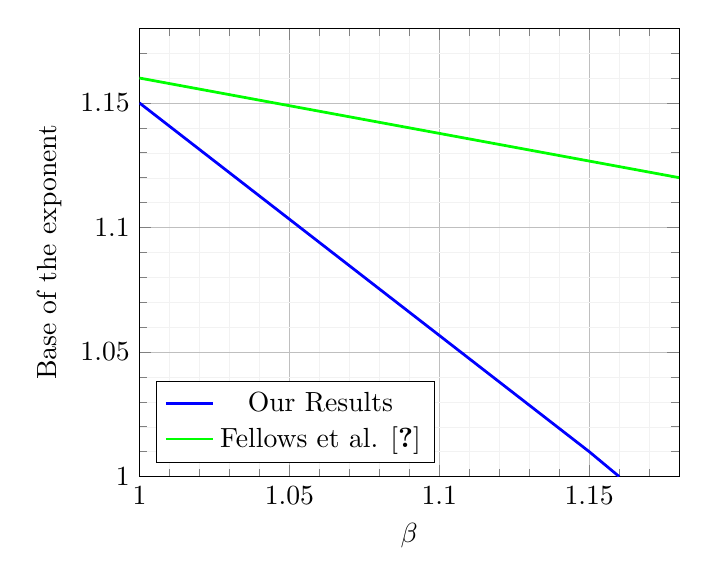
\begin{tikzpicture}
  \begin{axis}[
    xlabel={$\beta$},
    ylabel={Base of the exponent},
    xmin=1, xmax=1.18,
    ymin=1, ymax=1.18,
    grid=both,
    grid style={line width=.1pt, draw=gray!10},
    major grid style={line width=.2pt,draw=gray!50},
    minor tick num=4,
    legend style={at={(0.03,0.03)}, anchor=south west}
  ]
  
  % Our Results line
  \addplot[
    color=blue,
    mark=none,
    line width=1pt
  ] coordinates {
    (1, 1.15)
    (1.15, 1.01)
    (1.16, 1)
  };
  
  % Fellows et al. line
  \addplot[
    color=green,
    mark=none,
    line width=1pt
  ] coordinates {
    (1, 1.16)
    (1.18, 1.12)
  };
  
  \legend{Our Results, Fellows et al. \cite{?}}
  \end{axis}
\end{tikzpicture}

\end{document}